\chapter{Discussion}

\section{Scan settings}
Selecting acceptable settings is a compromise between resolution, signal, noise and time. As water evaporates rather quick (maximum evaporation time was found to be an hour), scanning a whole slide in one job is not possible with any of the water objectives. This leaves us left with the 20x dry and 63x oil objective. As seen in table \ref{tab:obj_time} using 63x oil objective a scan job will take about twice as long as with a 20x dry objective. This was found to be an acceptable trade off between time and resolution, with a whole scan taking minimum two hours.

As we can see in figure \ref{fig:obj_comparison}, we have weaker signal with the 63x water objective compared to 20x dry. Although the gain of the detector is 50 Volt higher in image (a), this should not give difference of such magnitude. As a lot of things will effect the intensity, ranging all the way from laser power to mirror oscillation frequency, one should confirm the intensity range by taking a small test scan before scanning a whole slide.

One factor that is limiting to laser power, is HyD detector shutting down due getting several photons at the same time. A good solution to this problem has not been found. Limiting laser power will decrease amount of bright spots which is able to shut down HyD detector, but the problem is not completely excluded until setting laser power too low to generate any significant signal. It is suggested that one concentrate on forward PMT detectors until one can eliminate bright spots.

\section{Automation of the process}
Tile scan give limited options to adjusting a scan and also makes it hard to separate samples. Using matrix scan is therefor more appropriate for scanning slides where samples are spread over a large area. Also, a feature in the software called \textit{computer assisted microscopy} may be used for automatic adjusting of placement to wells.



\section{Quantification}

\subsection{Gradient}
Using gradient for quantifying fiber direction does not seem to be a good match. This is illustrated in figure \ref{fig:grad} and \ref{fig:grad_arr}, where a lot of random directions get generated. Especially angles which are multiples of 45 degrees get a high response, which is due to the nature of the data (being a two dimensional image). As one might imagine, a single pixel of high intensity (as noise often is), would generate gradients with magnitude of n$\cdot$45 degrees in the pixels around. This is not easily remedied with filtering, as one would simply create a "mountain" where the strong pixel is (and get the same effect further away from the pixel).

\begin{figure}[h]
\centering
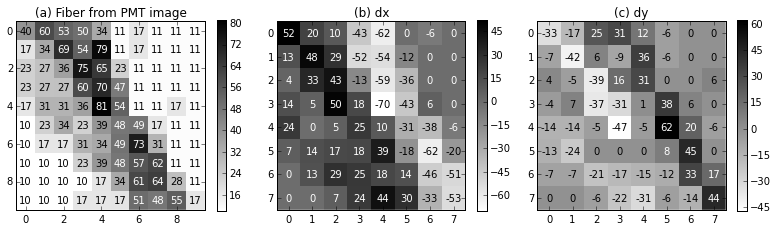
\includegraphics[width=\textwidth]{gradient}
\caption{(a) Section of image with strong signal from a fiber. Numbers in cells are intensity values of image. (b) X-component of gradient. (c) Y-component of gradient.}
\label{fig:grad}
\end{figure}

\begin{figure}[H]
\centering
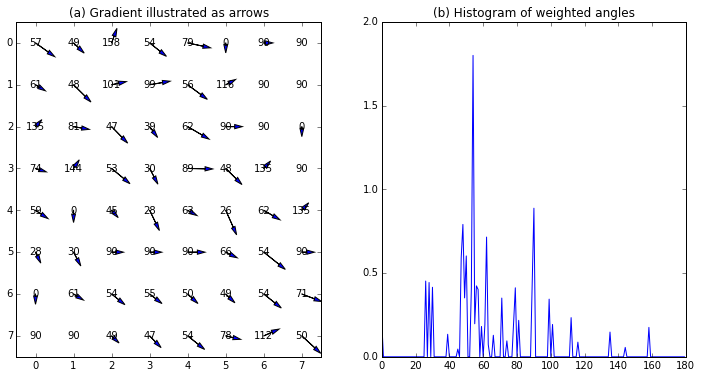
\includegraphics[width=\textwidth]{gradient_arrow}
\caption{(a) Gradient to image in figure \ref{fig:grad} (a) drawn as arrows. An angle of 90 degrees have been added to gradient to align the gradient in the same direction as the fiber. (b) The weighed histogram of angles to gradients in (a).}
\label{fig:grad_arr}
\end{figure}

A possible improvement could be to discard all but the strongest or averaged direction to gradients of sub images. Also, one could try to preprocess the image with some kind of edge detection and then using similar technique on a binary image.


\subsection{Frequency domain}
Line fitting of sub images in the Fourier image give good indication of strong fiber orientations. Lines with low correlation coefficient, as in figure \ref{fig:line_bad}, should be discarded to not include angles which are merely selected at random. A possibility to improve this technique is summing up angles instead of using line fit.

\begin{figure}[h]
\centering
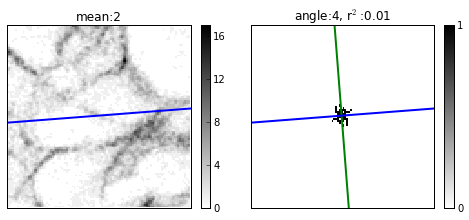
\includegraphics[width=0.66\textwidth]{ft_line_bad}
\caption{(a) Sub image of a sample. (b) Fourier spectrum and line fit. Note the low correlation coefficient r$^2$ = 0.01.}
\label{fig:line_bad}
\end{figure}

Summing up angles of highest intensities in Fourier spectrum seem to be good approach in detecting direction of fibers in image. In the images selected, the broadness of the peak in the histogram is a good measure of fiber direction anisotropy. This should be verified on a larger data set. One problem might be directions with similar angles, which may overlap in the histogram and broadening the peak. A possible solution to this is dividing the image into sub images as the previous Fourier algorithm.